\documentclass[a4paper,11pt]{article}
\usepackage{indentfirst}  % Indente aussi le premier paragraphe après chaque section
\usepackage{amsmath}
\usepackage{amssymb}  % Pour \mathbb et les symboles mathématiques supplémentaires
\usepackage{graphicx}
\usepackage{geometry}
\geometry{margin=1in}
\usepackage{booktabs}
\usepackage{hyperref}
\usepackage[utf8]{inputenc}
\usepackage[T1]{fontenc}

\setlength{\parindent}{1cm}

\title{You Only Look Once (Yolo)}
\author{BEX Roméo, RIVALDI Tristan, LAMURE Maxence}
\date{24 Septembre 2024}

\begin{document}

\begin{titlepage}

    \begin{minipage}{0.3\linewidth}
     
\includegraphics[width=0.70\textwidth]{../Images/logo_univ.png}   
    \end{minipage}
    \begin{minipage}{0.7\linewidth}
    \LARGE
            \textbf{Université de Montpellier} 
    \end{minipage}
    
    \begin{minipage}{0.3\linewidth}
     
\includegraphics[width=0.60\textwidth]{../Images/logoSSD.png}   
    \end{minipage}
    \begin{minipage}{0.7\linewidth}
    \LARGE
            \textbf{Master 2 Statistiques et Sciences des Données}        
    \end{minipage}
    
    \vspace*{1cm}
    
        \begin{center}
         
            \Huge
    
    \hrulefill
            
            \textbf{You Only Look Once (Yolo)}
    
    \hrulefill

            \vspace{0.5cm}
                
            \large
            \href{https://github.com/RomeoBex/Yolo}{\texttt{https://github.com/RomeoBex/Yolo}}
        
                
                        
            \vspace{2cm}
    
            \Large
            \begin{minipage}[t]{0.4\textwidth}
                 \textbf{Auteurs :}
            \end{minipage}
            \hfill
            \begin{minipage}[t]{0.45\textwidth}
                \raggedleft
                BEX Roméo\\
                RIVALDI Tristan\\ 
                LAMURE Maxence
            \end{minipage}
                
                
            \vspace{9cm}
            \large
            2024 - 2025
                
        \end{center}
    \end{titlepage}

\newpage

\tableofcontents

\newpage

\section{Introduction}

\indent L’article \textit{You Only Look Once: Unified, Real-Time Object Detection} présente une approche unifiée pour la détection d’objets en temps réel. YOLO (You Only Look Once) reformule la tâche de détection comme un problème de régression directe, reliant l’image complète aux coordonnées des boîtes englobantes et aux probabilités de classes. Contrairement aux méthodes traditionnelles, telles que R-CNN, qui découpent le processus en plusieurs étapes (propositions, classification), YOLO effectue toutes les prédictions en une seule évaluation. Ce gain de simplicité structurelle se traduit par une exécution extrêmement rapide, offrant des applications potentielles dans des domaines exigeants tels que la conduite autonome, la robotique, et la surveillance.

\section{Méthodologie}

\indent YOLO adopte un pipeline simple mais efficace pour la détection d'objets. Premièrement, l'image d'entrée, quelle que soit sa résolution initiale, est redimensionnée à une taille fixe de 448x448 pixels. Ce redimensionnement standardise le traitement en garantissant que toutes les images aient les mêmes dimensions, facilitant ainsi une évaluation rapide et cohérente.

Ensuite, l'image est divisée en une grille de taille $S \times S$, chaque cellule de la grille étant responsable de prédire plusieurs boîtes englobantes ainsi que les scores de confiance associés. En plus des coordonnées des boîtes, une carte des probabilités de classe est également générée, assignant des probabilités à chaque classe possible dans chaque cellule. Enfin, les boîtes englobantes finales sont ajustées pour représenter avec précision les objets détectés, comme le chien, la bicyclette et la voiture dans la Figure \ref{fig:yolo}.

\begin{figure}[h!]
    \centering
    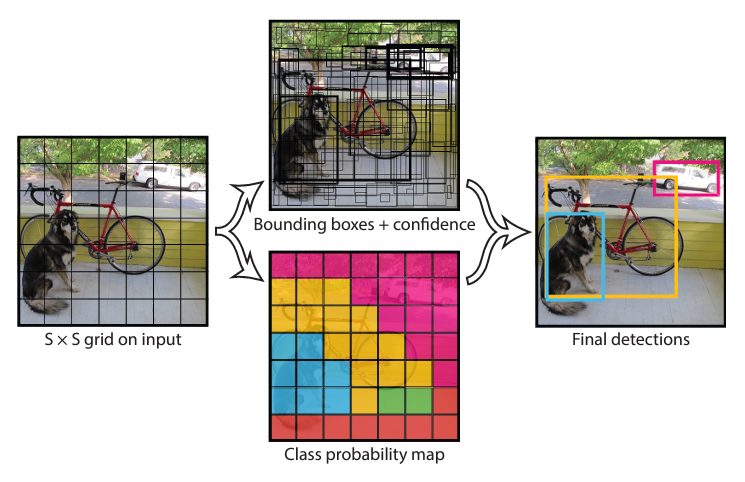
\includegraphics[width=0.8\textwidth]{../Images/yolo_architecture.PNG}
    \caption{Illustration du processus de détection d'objets avec YOLO.}
    \label{fig:yolo}
\end{figure}
    

\subsection{Formulation du problème}

\indent La détection d'objets dans YOLO est formulée comme un problème de régression. Le modèle prédit directement les coordonnées des boîtes englobantes $(x, y, w, h)$, où $(x, y)$ sont les coordonnées du centre de la boîte par rapport à la cellule de la grille, et $(w, h)$ sont la largeur et la hauteur de la boîte par rapport à l'image entière.

Pour estimer la qualité de la prédiction, YOLO introduit une notion de confiance, qui combine la probabilité de la classe prédite et l'IoU (\textit{Intersection over Union}) entre la boîte prédite et la boîte réelle (ground truth). La confiance pour chaque boîte est donnée par :
\[
P(Class_i|Object) \times P(Object) \times IoU_{\text{truth, pred}} = P(Class_i) \times IoU_{\text{truth, pred}}.
\]
\indent Cette équation combine la probabilité qu’un objet soit présent et l’IoU entre la boîte prédite et la boîte réelle. Ainsi, la confiance reflète à la fois la probabilité qu’une classe d’objet soit présente et la précision de la localisation de l’objet.

\subsection{Structure du réseau YOLO}

\indent YOLO repose sur un réseau convolutif profond inspiré par GoogLeNet, comprenant 24 couches convolutionnelles suivies de deux couches entièrement connectées. Ce modèle traite l'image entière en une seule passe, générant un tenseur de taille $S \times S \times (B \times 5 + C)$, où $B$ représente le nombre de boîtes englobantes prédites par cellule, et $C$ le nombre de classes. Les prédictions incluent les coordonnées des boîtes, les scores de confiance, et les probabilités de classes.

\subsection{Fonction de perte}

\indent La fonction de perte utilisée pour entraîner YOLO joue un rôle crucial dans ses performances. Elle combine plusieurs composantes pour optimiser simultanément la localisation des boîtes et la classification des objets.

La fonction de perte totale peut s'écrire sous la forme suivante :
\[
\lambda_{\text{coord}} \sum_{i=0}^{S^2} \sum_{j=0}^{B} 1^{\text{obj}}_{ij} \underbrace{\left[(x_i - \hat{x}_i)^2 + (y_i - \hat{y}_i)^2\right]}_{\text{Erreur de localisation}}
+ \lambda_{\text{coord}} \sum_{i=0}^{S^2} \sum_{j=0}^{B} 1^{\text{obj}}_{ij} \underbrace{\left[\left(\sqrt{w_i} - \sqrt{\hat{w}_i}\right)^2 + \left(\sqrt{h_i} - \sqrt{\hat{h}_i}\right)^2 \right]}_{\text{Erreur de taille (largeur/hauteur des boîtes)}}
\]
\[
+ \sum_{i=0}^{S^2} \sum_{j=0}^{B} 1^{\text{obj}}_{ij} \underbrace{\left(C_i - \hat{C}_i\right)^2}_{\text{Erreur avec objet}} 
+ \lambda_{\text{noobj}} \sum_{i=0}^{S^2} \sum_{j=0}^{B} 1^{\text{noobj}}_{ij} \underbrace{\left(C_i - \hat{C}_i\right)^2}_{\text{Erreur sans objet}}
\]
\[
+ \sum_{i=0}^{S^2} 1^{\text{obj}}_i \sum_{c \in \text{classes}} \underbrace{\left(p_i(c) - \hat{p}_i(c)\right)^2}_{\text{Erreur de classification}}
\]

\noindent Cette fonction de perte se compose de plusieurs termes :
\begin{itemize}
    \item Le premier terme concerne l'erreur de localisation $(x, y)$ des boîtes prédictes.
    \item Le second terme optimise la largeur et la hauteur $(w, h)$ des boîtes prédictes. Le fait de prendre la racine carrée des dimensions permet de réduire l'impact des grandes boîtes sur la fonction de perte.
    \item Le troisième terme minimise l'erreur sur la confiance associée aux boîtes contenant des objets.
    \item Le quatrième terme pondère l'erreur de confiance pour les cellules qui ne contiennent pas d’objets, afin d’éviter que ces cellules ne dominent la fonction de perte (grâce à un hyperparamètre $\lambda_{\text{noobj}}$ plus faible).
    \item Enfin, le dernier terme traite la classification des objets à l'intérieur des boîtes.
\end{itemize}

Cette fonction de perte complexe permet à YOLO de mieux gérer les cas où les objets sont absents, en réduisant les faux positifs et en améliorant la précision globale de la détection.

\section{Comparaison des méthodes}

\indent YOLO se distingue des autres méthodes de détection par sa rapidité d'exécution, bien qu'il présente une légère baisse de précision par rapport à certaines méthodes traditionnelles. Par exemple, sur le jeu de données PASCAL VOC 2007, YOLO atteint un mAP (mean Average Precision) de 63,4 \%, comparé à 73,2 \% pour Faster R-CNN. Cependant, YOLO compense cette baisse de précision par une vitesse nettement supérieure, avec 45 FPS contre 7 FPS pour Faster R-CNN.

\begin{table}[h]
\centering
\begin{tabular}{lcc}
\toprule
\textbf{Méthode} & \textbf{mAP (\%)} & \textbf{FPS} \\
\midrule
Fast R-CNN & 70.0 & 0.5 \\
Faster R-CNN & 73.2 & 7 \\
YOLO & 63.4 & 45 \\
Fast YOLO & 52.7 & 155 \\
\bottomrule
\end{tabular}
\caption{Comparaison des performances de détection sur PASCAL VOC 2007.}
\end{table}

\section{Limites et Faiblesses}

\indent Bien que YOLO présente des avantages indéniables en termes de vitesse, il comporte certaines limites. Premièrement, la localisation des objets, en particulier pour les petits objets proches des bords de l’image, est souvent moins précise. Cela est dû au fait que chaque cellule de la grille $S \times S$ ne peut prédire qu’un nombre limité de boîtes, ce qui peut affecter les objets de petite taille.

De plus, les petites erreurs dans la prédiction des dimensions des boîtes peuvent avoir un impact disproportionné sur l'IoU, ce qui pénalise davantage la performance globale du modèle pour les petits objets. Enfin, bien que YOLO généralise relativement bien sur des images naturelles, il peut rencontrer des difficultés à reconnaître des objets dans des configurations visuelles ou des proportions inhabituelles.

\section{Conclusion}

\indent YOLO propose une solution innovante en simplifiant le pipeline traditionnel de la détection d’objets, permettant ainsi une exécution en temps réel avec une bonne précision. Bien qu’il présente des limitations en termes de localisation, ses avantages en termes de rapidité et de généralisation font de YOLO une option attrayante pour des applications nécessitant une détection rapide, comme la robotique, la surveillance, et la réalité augmentée.

\end{document}
